% Multiple Choice Question 9 to 10 (2 questions)

\textbf{See the instruction for questions \inteval{\value{question}+1} to \inteval{\value{question}+2}.} 

\begin{center}
    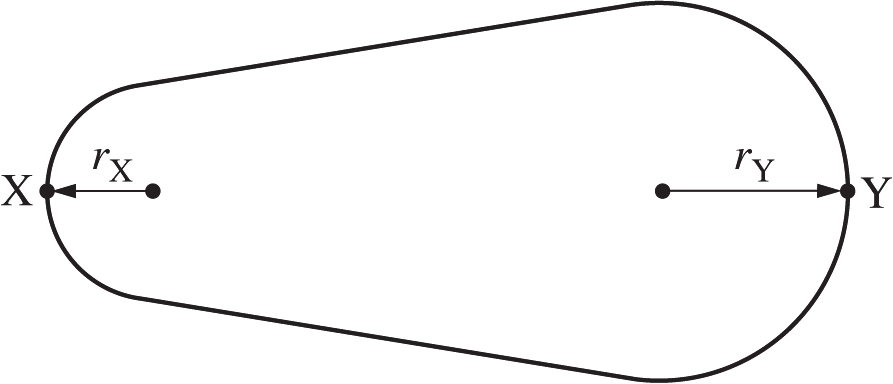
\includegraphics[scale=0.3]{images/img-006-006.png}
\end{center}

The figure above shows a cross section of a solid, isolated, metallic conductor in electrostatic equilibrium with a net charge $+Q$. The two ends of the conductor are spherical surfaces of radii $r_{\mathrm{X}}$ and $r_{\mathrm{Y}}$, where $r_{\mathrm{X}}<r_{\mathrm{Y}}$. Points $\mathrm{X}$ and $\mathrm{Y}$ are on the conductor at each end.

\begin{questions}
\setcounter{question}{8}

% Multiple Choice Question 9
\question
Assuming that the electric potential is zero an infinite distance from the conductor, which of the following statements is true about the magnitude of the electric potential at points $X$ and $Y$?

\begin{choices}
    \choice It is greater at point $X$ than at point $Y$.
    \choice It is greater at point $Y$ than at point $X$.
    \choice It is zero at both points $X$ and $Y$.
    \choice It has the same nonzero value at both points $X$ and $Y$.
    \choice There is not enough information to determine at which point, if either, the magnitude of the electric potential is greater.
\end{choices}

% Multiple Choice Question 10
\question
Which of the following is true about the magnitude of the electric field just outside the surface of the conductor at points $X$ and $Y$?

\begin{choices}
    \choice It is greater at point $X$ than at point $Y$.
    \choice It is greater at point $Y$ than at point $X$.
    \choice It is zero at both points $X$ and $Y$.
    \choice It has the same nonzero value at both points $X$ and $Y$.
    \choice There is not enough information to determine at which point, if either, the magnitude of the electric field is greater.
\end{choices}

\end{questions}
